\documentclass[11pt, abstracton]{scrartcl}

\usepackage[ngerman]{babel}
\usepackage[T1]{fontenc}
\usepackage[utf8]{inputenc}
\usepackage{lmodern}
\usepackage{graphicx}
\usepackage{amsmath}
\usepackage{amssymb}
\usepackage{biblatex}	
	

\title{Probabilistische Algorithmen}
\subtitle{Seminar Theoretische Informatik}
\author{Thorsten Kober}
\date{16. Juni 2015}


\bibliography{Bibliography}	

\begin{document}

\maketitle

\tableofcontents
\printbibliography
\pagebreak

\section{Einführung}


\subsection{Definition}
Unter einem probabilistischen (lat. \emph{probabilis} etwa \emph{glauben, wahrscheinlich}) Algorithmus versteht man ein Verfahren, welches mittels zufälligen Zwischenergebnissen versucht zu einer guten Näherung für ein korrektes Ergebnis zu gelangen.
Er bildet damit das Gegenstück zu einem deterministischen Algorithmus.


\subsection{Hintergrund}	
Es gibt Probleme deren Lösung durch mittels Nichtdeterminismus Vorteile hat, weil:
\begin{itemize}
	\item mit einer deterministischen Umsetzung eine zu Große Laufzeit einhergeht
	\item die Lösung nur \emph{hinreichend gut} und nicht optimal sein muss
	\item eine nichtdeterministische Lösung einfacher zu verstehen oder zu implementieren ist
	\item der Algorithmus nicht deterministische umzusetzen ist
\end{itemize}

Als kleine Motivation jetzt ein Beispiel für einen Algorithmus, dessen probabilistische Umsetzung effizienter ist als eine deterministische. 

\subsection{Beispiel: Quicksort}
\paragraph{Wiederholung:}
Die Vorgehensweise des Quicksort-Algorithmus ist prinzipiell folgende:
\begin{enumerate}
	\item Wähle aus einer Liste unsortierter Elemente eines aus (Pivotelement). Dieses Pivotelement stellt für sich eine einelementige vollständig sortierte Liste da.
	\item Vergleiche alle anderen Elemente der Liste mit dem Pivotelement und füge sie einer neuen Liste $L$ hinzu falls sie kleiner sind als das Pivotelement. Ansonsten füge sie der Liste $R$ hinzu.
	\item Führe Schritt 1 nun mit $L$ und $R$ durch. Enthält eine Liste nur noch ein Element endet der Algorithmus.
	\item Füge die Teillisten nun so zusammen, dass $L$ immer links des jeweiligen Pivotelements steht und $R$ rechts davon. Die resultierende Liste ist nun vollständig aufsteigend sortiert. Absteigend analog mit invertiertem Ordnungskriterium. 
\end{enumerate}

\begin{figure}[h]
	\centering
	\begin{minipage}{.45\textwidth}
		\centering
		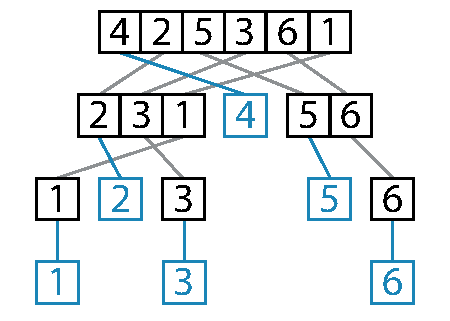
\includegraphics[width=\textwidth]{Graphics/Quicksort_example_avg}
	\end{minipage}
	\begin{minipage}{.45\textwidth}
		\centering
		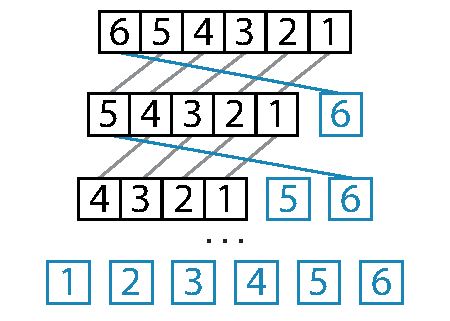
\includegraphics[width=\textwidth]{Graphics/Quicksort_example_wcet}
	\end{minipage}
	\caption{Beispiel für durchschnittliche(links) und schlechteste(rechts) Ausführungszeit eines primitiven Quicksort}
	\label{fig:quicksort_example}
\end{figure}

\paragraph{Beobachtung:}
Die Laufzeit des Quicksort-Algorithmus hängt maßgeblich von der Wahl des Pivotelements ab:
\begin{itemize}
	\item \textbf{Best-Case:} Das Pivotelement wird so gewählt, dass gilt $||L| - |R| | \leq 1$. Daraus ergibt sich mit $log(n)$ Schritten mit je $n$ Vergleichen eine Laufzeit von $\mathcal{O}(nlog(n))$.
	\item \textbf{Worst-Case:} Das Pivotelement wird so gewählt, dass gilt $|L| = 1$ oder $|R| = 1$. Daraus ergibt sich mit $n$ Schritten und je $n$ Vergleichen eine Laufzeit von $\mathcal{O}(n^2)$.
\end{itemize}


\paragraph{Lösung:}
Wird für jede n-elementige Teilliste das Pivotelement zufällig gewählt, beträgt die Wahrscheinlichkeit das schlechteste Element zu wählen $P(schlechtestes\ Element\ gewählt) = \frac{1}{n}$.
Selbiges gilt zwar auch für den \emph{Best-Case}, allerdings lässt sich zeigen, dass die Laufzeit der probabilsitischen Variante im Durchschnitt ebenfalls $\mathcal{O}(nlog(n))$ beträgt. \cite{knuth}









\section{Probabilistische Turingmaschinen}

\subsection{Definition}
Wir nutzen das Modell der Mehrband-Turingmaschine um abstrakt die Fähigkeit einer Turing-Maschine zu zeigen, eine zufällige Auswahl zu treffen, entsprechend einem Programm, das einen Zufallszahlengenerator einmal oder mehrfach aufruft.
Auf dem ersten Band steht wie bei einer Mehrband-Turingmaschine üblich die Eingabe.
Das zweite Band, das sogenannte \emph{Zufallsband}, ist vollständig mit den Symbolen $1$ und $0$, die zufällig und unabhängig voneinander mit der Wahrscheinlichkeit $P(x) = \frac{1}{2}, x \in \{0, 1\}$.
Die übrigen Bänder sind initial leer und können nach Bedarf als \emph{Hilfsbänder} genutzt werden.

\begin{figure}[h]
	\centering
	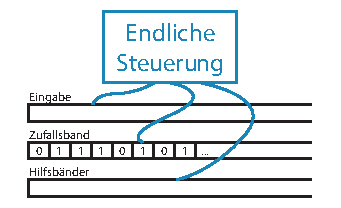
\includegraphics[width=.8\textwidth]{Graphics/Probabilistic_TM}	
\end{figure}

Wir nennen dieses Modell einer Turingmaschine \emph{zufallsabhängige Turingmaschine} oder \emph{probabilistische Turingmaschine}.


\subsection{Initialisierung des Zufallsbandes}
\paragraph{Beobachtung:}
Da die komplette Initialisierung des unendlichen Zufallsbandes mit den Symbolen $1$ und $0$ ist nicht realistisch, da diese nie terminiert.

\paragraph{Lösung:}
Das Zufallsband ist initial ebenfalls leer, enthält also nur \emph{Blanks}. 
Liest der Lese-Schreibkopf auf dem Zufallsband nun ein \emph{Blank}, so wird intern mittels eines Zufallsgenerators eine $1$ oder eine $0$ erzeugt und auf das Zufallsband geschrieben.
Das generierte Symbol wird anschließend nicht wieder verändert.
Auf diese Weise scheint das Zufallsband vollständig initialisiert.

\subsection{Beispiel: Probabilistischer Quicksort}


\subsection{Sprache}
\section{Probabilistische Komplexitätsklassen}


\subsection{Wiederholung: Zeitkomplexität}


\subsection{RP}


\subsection{BPP}


\subsection{ZPP}
\section{Beziehungen zwischen RP, BPP und ZPP}
\section{Beziehungen von probabilistischen Komplexitätsklassen zu P und NP}

\end{document}
